% !TEX root = deplump.tex
\section{Experiments}
\label{sec:experiments}
The performance and characteristics of Deplump were investigated using the most recent Wikipedia content dump as a test corpus.  As a preliminary analysis, we ran the algorithm twice on the first 100Mb section of the corpus with the depth limited to 16 and 1024.  At the end of the section, the depth and total count was printed at each non-leaf node for each suffix tree.  The scatter plots in Figure~\ref{fig:restaurant_plots} show 100,000 randomly sampled points from this output for each tree.  The fact that there are very few nodes with high total counts suggested that we could set the count upper bound fairly low.  As a follow up experiment we used the algorithm with $L$ set to a million, the depth set to 16, and $k$ varied from 128 to 32,768, to compress ten 100MB subsections of the corpus, sampled randomly with replacement.  Average compression performance varied only slightly across values of $k$.

We then investigate empirical performance for other values in of the model parameters.  Performance is measured in bits per byte, which can be converted to compression ratio by dividing by eight.  For each setting of the parameters, ten sections of the corpus were sample with replacement from the corpus and compressed using the algorithm.  In the first sets of experiments, the sampled subsection was 100Mb, while in the second the sampled subsection varied in length.  In the first set of experiments, $k$ was fixed to 8,192, while $L$ and the depth of the tree were varied. Results are shown in Figure~\ref{fig:varying_depths}. In the second set of experiments $k$ was set to 8,192 and the depth was set to 16 while $L$ was allowed to vary.  Results from the third set of experiments are shown in Figure~\ref{fig:varying_stream_length}.

Figure~\ref{fig:varying_depths} indicates that performance stops improving for depths larger than 10 or 12 while controlling for $L$.  This figure also makes it clear that performance is improved with a larger number of nodes in the tree as long as the depth is at least 6.  Figure~\ref{fig:varying_stream_length} illustrates that the algorithm not only scales to very long sequences, but continues to improve as the sequence grows.  Using a large value of $K$ appears to be beneficial for very long sequences.

\begin{figure*}[t] 
	\begin{center}
		\scalebox{.6}{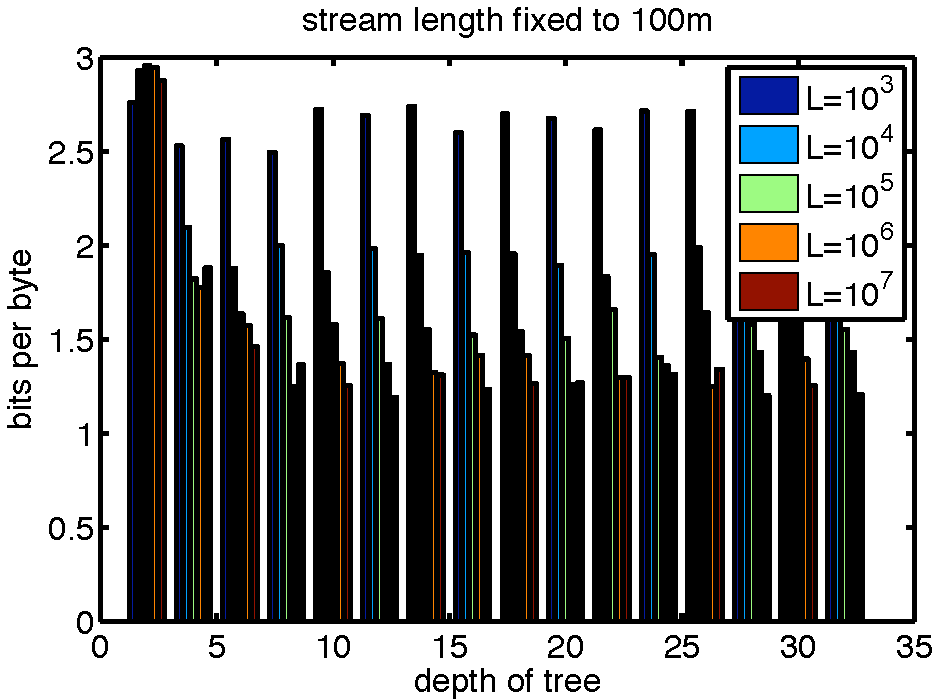
\includegraphics{figs/varying_depths.pdf}} % [clip=true, viewport= 1in 1in 9in 9in]
		\caption{Performance averaged over 10 random sections  100Mb sections of the corpus for varying fixed depths and number of allowable nodes ($L$) }
		\label{fig:varying_depths}
	\end{center} 
\end{figure*} 

%\begin{figure*}[t] 
%	\begin{center}
%		\scalebox{.6}{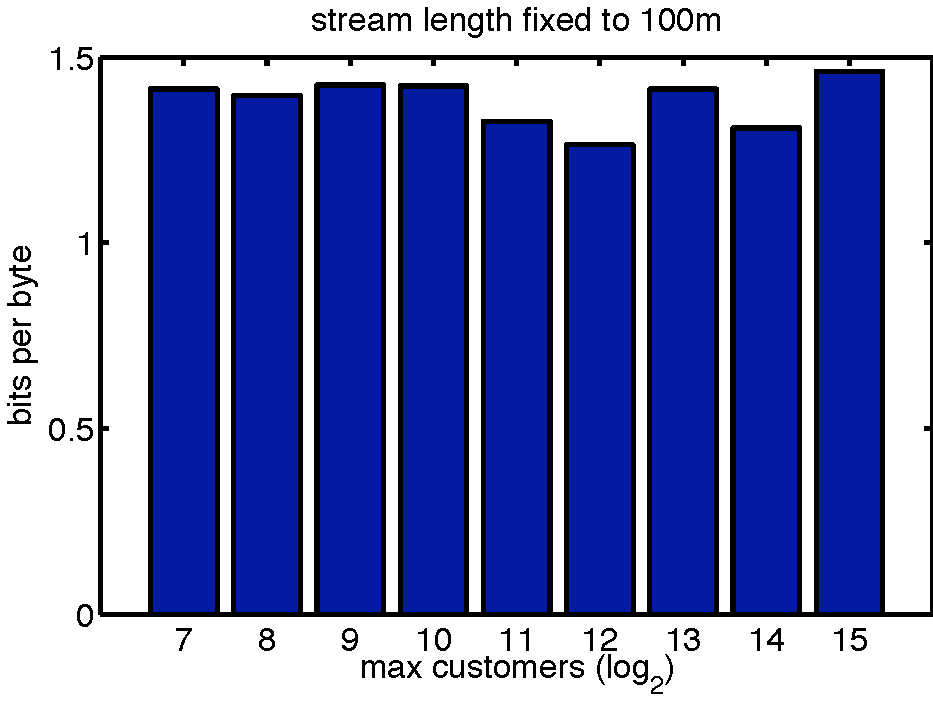
\includegraphics{figs/varying_max_customers.pdf}} % [clip=true, viewport= 1in 1in 9in 9in]
%		\caption{Performance for varying max allowable customers $k$.}
%		\label{fig: varying_max_customers}
%	\end{center} 
%\end{figure*} 

\begin{figure*}[t] 
	\begin{center}
		\scalebox{.6}{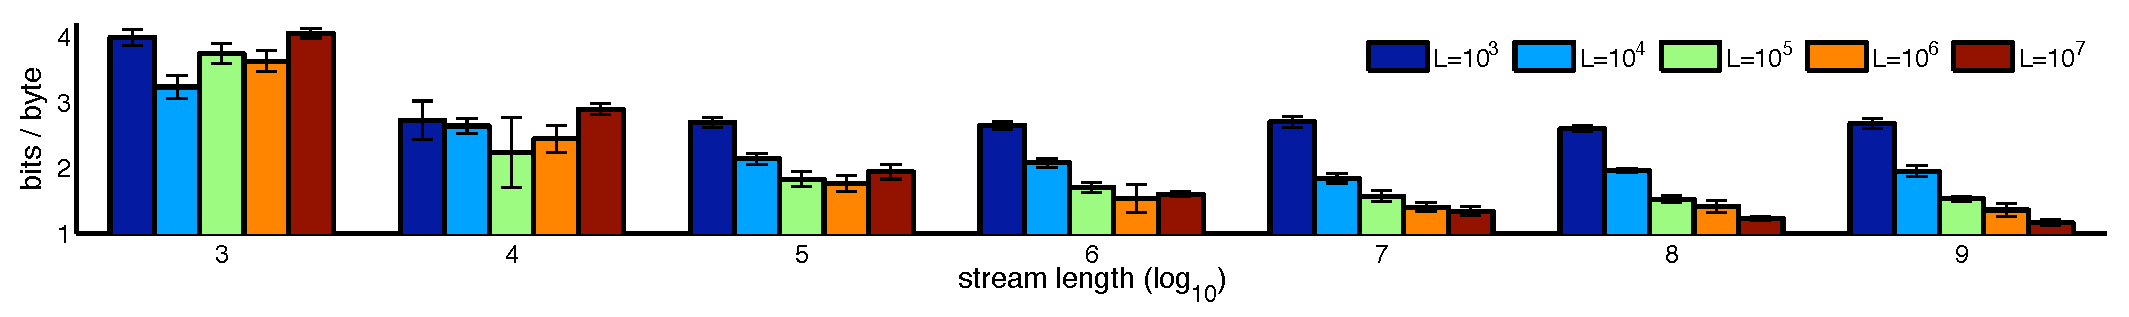
\includegraphics{figs/varying_stream_length.pdf}} % [clip=true, viewport= 1in 1in 9in 9in]
		\caption{Performance for varying stream lengths and number of allowable nodes ($L$).}
		\label{fig:varying_stream_length}
	\end{center} 
\end{figure*} 

\begin{figure*}[t] 
	\begin{center}
		\scalebox{1}{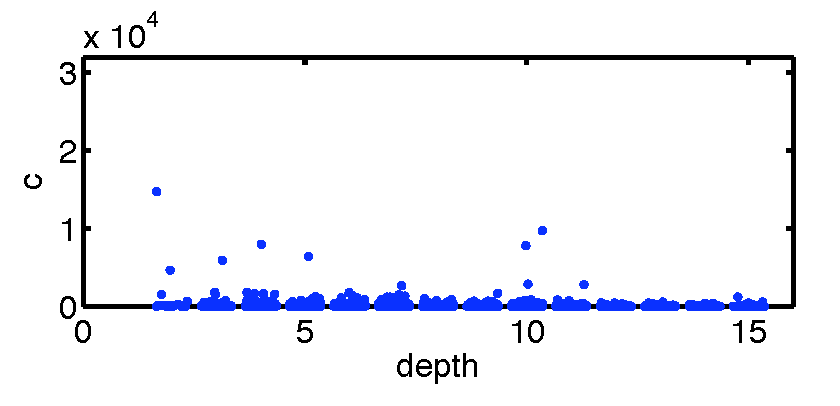
\includegraphics{figs/scatter_16.pdf}} % [clip=true, viewport= 1in 1in 9in 9in]
		\caption{Scatter plots to explore the relationship between the depth of a node and the total count}
		\label{fig:restaurant_plots}
	\end{center} 
\end{figure*} 

\begin{figure*}[t] 
	\begin{center}
		\scalebox{1}{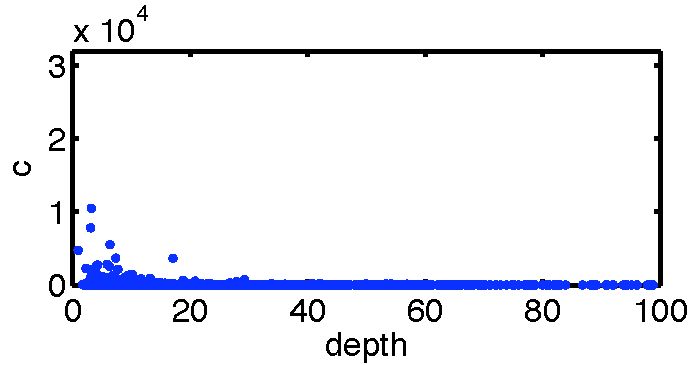
\includegraphics{figs/scatter_1024.pdf}} % [clip=true, viewport= 1in 1in 9in 9in]
		\caption{Scatter plots to explore the relationship between the depth of a node and the total count}
		\label{fig:restaurant_plots}
	\end{center} 
\end{figure*} 
